\begin{samplecase}
{\bf Residual production cross sections for protons on Fe}\newline
In this sample case, we calculate the residual production cross sections for
protons on ${}^{nat}$Fe for incident energies up to 100 MeV. A calculation for
a natural target is launched, meaning that successive TALYS calculations for
each isotope are performed, after which the results are weighted with the
natural abundance. We restrict ourselves to a calculation with all
nuclear model parameters set to their default values.
The following input file is used:

\VerbatimInput{\samples p-Fe000-rp/org/talys.inp}

The file {\em energies} contains 24 incident energies between 1 and 100 MeV.
Obviously, this sample case can be extended to more incident energies, e.g. up
to 200 MeV, by simply adding numbers to the {\em energies} file. In that case,
we recommend to include more energy bins in the
calculation, (e.g. {\bf bins 80}) to avoid numerical fluctuations, although
this will inevitably take more computer time.
Note that we have enabled the {\bf fileresidual} keyword, so that a separate
cross sections file for each final product is produced.
The results from the files {\em rp027056.tot}, {\em rp027055.tot},
{\em rp025054.tot} and {\em rp025052.tot} are
presented, together with experimental data, in Fig.~\ref{resprod}.

As an example, the file {\em rp025052.tot} looks as follows.
{\small \begin{verbatim}
# header:
#   title: Fe0(p,x)Mn52 cross section
#   source: TALYS-2.0
#   user: Arjan Koning
#   date: 2023-12-11
#   format: YANDF-0.1
# target:
#   Z: 26
#   A: 0
#   nuclide: Fe0
# reaction:
#   type: (p,x)
#   ENDF_MF: 6
#   ENDF_MT: 5
# residual:
#   Z: 25
#   A: 52
#   nuclide: Mn52
# datablock:
#   quantity: cross section
#   columns: 2
#   entries: 24
##       E             xs
##     [MeV]          [mb]
   1.000000E+00   0.000000E+00
.....................
   1.600000E+01   0.000000E+00
   1.800000E+01   1.777641E-03
   2.000000E+01   4.415140E-01
   2.500000E+01   2.496402E+01
   3.000000E+01   3.582130E+01
   3.500000E+01   3.283743E+01
   4.000000E+01   2.765386E+01
   4.500000E+01   2.235001E+01
   5.000000E+01   1.994102E+01
   6.000000E+01   4.507320E+01
   7.000000E+01   6.835677E+01
   8.000000E+01   7.106861E+01
   9.000000E+01   6.800709E+01
   1.000000E+02   6.312850E+01
\end{verbatim} } \renewcommand{\baselinestretch}{1.07}\small\normalsize
\noindent
\end{samplecase}
\begin{figure}
\centering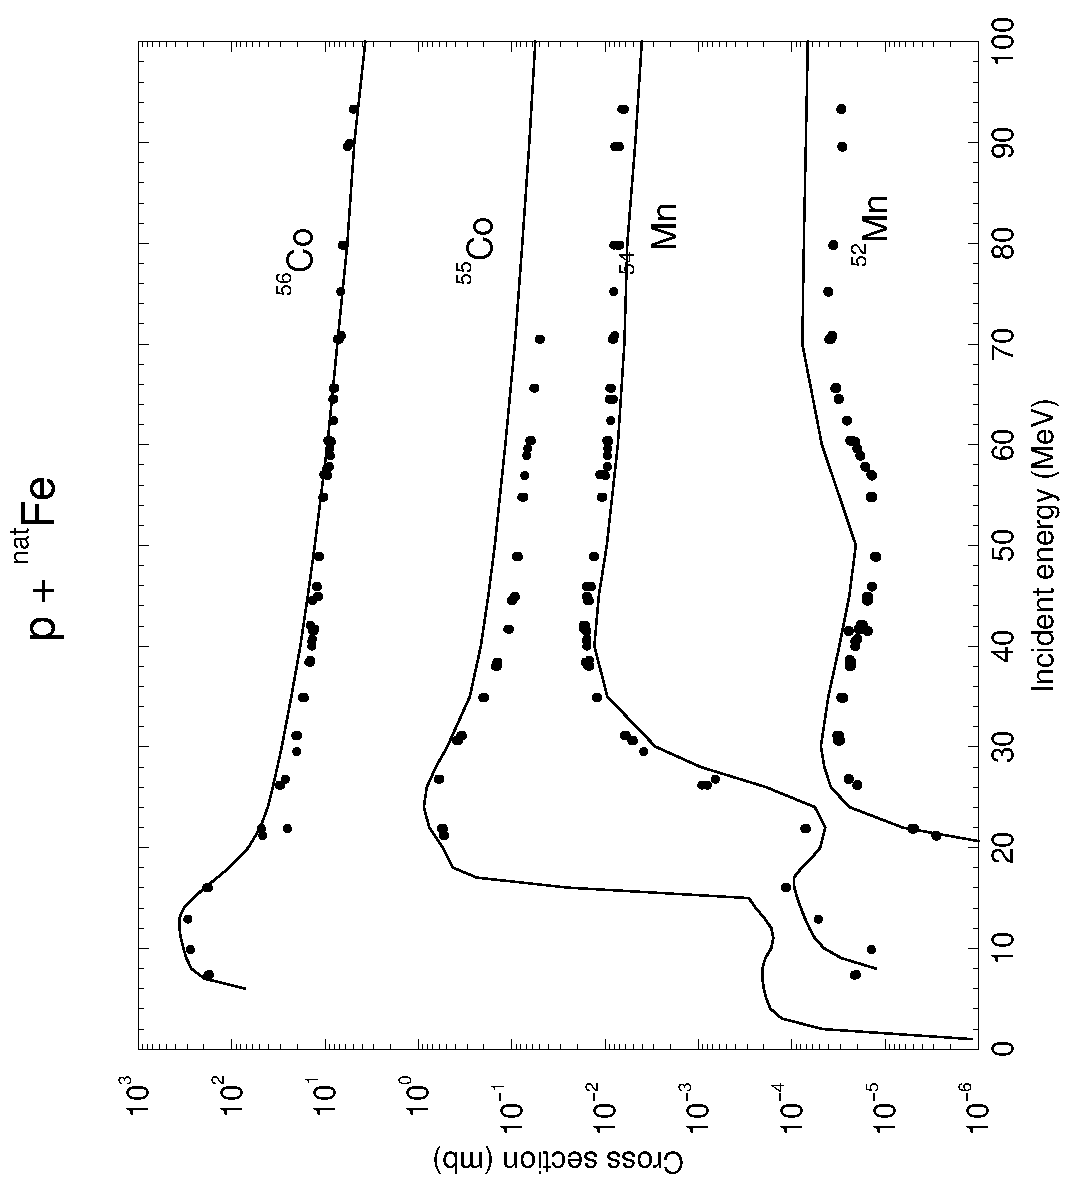
\includegraphics[scale=0.6,angle=270]{feresidual}
\caption{Residual production cross sections for protons incident
on ${}^{nat}$Fe. Experimental data are obtained from \protect\cite{Michel1997}.}
\label{resprod}
\end{figure}
